%----------------------------------------------------------------------------------------
%	PACKAGES AND THEMES
%----------------------------------------------------------------------------------------
\PassOptionsToPackage{table}{xcolor}
\documentclass[aspectratio=169,xcolor=dvipsnames,svgnames,x11names,fleqn]{beamer}
% \documentclass[aspectratio=169,xcolor=dvipsnames,fleqn]{beamer}

\usetheme{RedVelvet}

\usefonttheme[onlymath]{serif}
\newcommand{\showanswers}{yes}


\usepackage{xspace}
\usepackage{amsmath}
\usepackage{amssymb}
\usepackage{amsfonts}
\usepackage{color}
\usepackage{physics}
% \usepackage{mathbb}
\usepackage{rahul_math}
\usepackage{bigints}

\usepackage{graphicx} % Allows including images
\usepackage{booktabs} % Allows the use of \toprule, \midrule and \bottomrule in tables
\usepackage{tikz,pgfplots}

\usepackage{subfigure}
\usetikzlibrary{arrows}
\usepackage{minted}
\definecolor{LightGray}{gray}{0.9}
\definecolor{cream}{rgb}{0.92, 0.9, 0.55}
\definecolor{lightblue}{rgb}{0.68, 0.85, 0.9}


\usepackage{xcolor-material}
\usetikzlibrary{fit}
\usetikzlibrary{matrix}
\tikzset{%
apple/.pic={
    \fill [MaterialBrown] (-1/8,0)  arc (180:120:1 and 3/2) coordinate [pos=3/5] (@)-- ++(1/6,-1/7)  arc (120:180:5/4 and 3/2) -- cycle;
    \fill [MaterialLightGreen500] (0,-9/10)  .. controls ++(180:1/8) and ++(  0:1/4) .. (-1/3,  -1) .. controls ++(180:1/3) and ++(270:1/2) .. (  -1,   0) .. controls ++( 90:1/3) and ++(180:1/3) .. (-1/2, 3/4) .. controls ++(  0:1/8) and ++(135:1/8) .. (   0, 4/7)
    }
    }

\newcommand{\leftdoublequote}{\textcolor{blue}{\scalebox{3}{``}}}

\newcommand{\rightdoublequote}{\textcolor{blue}{\scalebox{3}{''}}}


\usepackage{textcomp}
\usepackage{fontawesome}
\usepackage{tikz,pgfplots}
\usetikzlibrary{shapes.callouts}
\usetikzlibrary{arrows}


\usepackage{overpic}

%----------------------------------------------------------------------------------------
%	TITLE PAGE
%----------------------------------------------------------------------------------------

\usepackage{tikz-qtree,tikz-qtree-compat}
\usetikzlibrary{tikzmark}
\usetikzlibrary{calc}


\title[CPE 486/586: Machine Learning]{CPE 486/586: Machine Learning for Engineers} % The short title appears at the bottom of every slide, the full title is only on the title page
\subtitle{12 Support Vector Machine}

\author[Rahul Bhadani] {{\Large \textbf{Rahul Bhadani}}}

\institute[UAH] % Your institution as it will appear on the bottom of every slide, maybe shorthand to save space
{
    Electrical \& Computer Engineering,  The University of Alabama in Huntsville
}
\date

% \titlegraphic{
%    \includegraphics[width=0.4\linewidth]{figures/UAH_primary.png}
% }

\begin{document}

%-------------------------------------------------
\begin{frame}
    \titlepage
\end{frame}

%-------------------------------------------------
\begin{frame}{Outline}
    \backgroundtableofcontents
\end{frame}




%%%%%%%%%%%%%%%%%%%%%%%%%%%%%%%%%%%%%%%%%%%%%%%%%%%%%
\begin{sectionframe}{\faCrop}{Constraint Optimization with Inequality}
\end{sectionframe}

\begin{frame}{Inequality Constraints}
    
    \Large
    \begin{center}
        $
        \min_x f(x) 
        $

        subject to 

        $
        g(x) \geq 0
        $
    \end{center}

    Without the constraint, $\cfrac{d f(x^*)}{dx} = 0$.

    With the inequality constraint, the solution lies either on the boundary, $g(x^*) = 0$ (the constraint is \emph{active}), or in the interior, $g(x^*) > 0$ (the constraint is \emph{inactive}, and $\cfrac{d f(x^*)}{dx} = 0$ still holds).
\end{frame}


\begin{frame}{Inequality Constraints with Lagrange Multiplier}

    \begin{center}
    We could still write the Lagrangian:

    \begin{multiequation}
        \Lcal (x,\lambda) & = f(x) - \lambda^\T g(x) \\
        \cfrac{\partial \Lcal}{\partial x}(x^*,\lambda^*) & = \cfrac{\partial f}{\partial x}(x^*) - \left(\cfrac{\partial g}{\partial x}(x^*)\right)^{\T}\lambda^* = 0 \quad \text{(stationarity)}\\
        g(x^*) & \geq 0 \quad \text{(primal feasibility)}\\
        \lambda^* & \geq 0 \quad \text{(dual feasibility)}\\
        \lambda^* \odot g(x^*) & = 0 \quad \text{(complementary slackness)}\\
            \end{multiequation}

    where $\odot$ is the element-wise product.

These conditions are called \textbf{Karush-Kuhn-Tucker Conditions} (KKT).

    \end{center}

\end{frame}

%------------------------------------------------
    \begin{frame}{The Generalized Lagrangian}
    \begin{tblock}{}
    The generalized Lagrangian function to {\color{MediumRed}minimize} $f(x)$ subject to equality constraints $g_i(x) = 0$ and inequality constraints $h_j(x) \leq 0$ is  
    \begin{multiequation}
    L(x, \lambda, \beta) = f(x) + \sum_{i=1}^I \lambda_i g_i(x) + \sum_{j=1}^J \beta_j h_j(x), \quad \beta_j \geq 0
    \end{multiequation}
    \end{tblock}
    
    \end{frame}


    
    
%------------------------------------------------
\begin{frame}{Karush-Kuhn-Tucker Conditions}
    \begin{itemize}
    \item If we have several equality and inequality constraints, in the following form
    \begin{multiequation}
    \arg\min_{x} f(x), \text{ s.t. } g_i(x) = 0, h_j(x) \leq 0
    \end{multiequation}
    The KKT conditions are necessary for optimality (under a constraint qualification). They are also sufficient when $f$ and $h_j$ are convex and $g_i$ are affine:
    \begin{multiequation}
    &\frac{\partial L(x^*, \lambda^*, \beta^*)}{\partial x} = 0, \hspace{1em}
    \frac{\partial L(x^*, \lambda^*, \beta^*)}{\partial \beta} = 0, \hspace{1em} 
    g_i(x^*) = 0, \hspace{1em}
    h_j(x^*) \leq 0, \\
    &\sum_{j=1}^J \beta_j^* h_j(x^*) = 0, \hspace{1em} 
    \beta_j^* \geq 0 \;\; (\lambda_i^* \text{ unrestricted in sign})
    \end{multiequation}
    Since the terms $\beta_j^* h_j(x^*)$ are nonpositive, $\sum_j \beta_j^* h_j(x^*) = 0$ is equivalent to $\beta_j^* h_j(x^*) = 0$ for $j = 1, \dots, J$.
    \end{itemize}
    \end{frame}
    
    
    %------------------------------------------------
    \begin{frame}{The Generalized Lagrangian}
    \begin{tblock}{}
    The generalized Lagrangian function to {\color{MediumRed}minimize} $f(x)$ subject to the equality constraints on $g_i(x)$ and inequality constraints on $h_j(x)$ is given by:  
    \begin{multiequation}
    L(x, \lambda, \beta) = f(x) + \sum_{i=1}^I \lambda_i g_i(x) + \sum_{j=1}^J \beta_j h_j(x)
    \end{multiequation}
    \end{tblock}
    
    \end{frame}
    

% https://home.cc.umanitoba.ca/~lovetrij/cECE7670/2005/Slides/slides7.pdf

% https://pweb.fbe.hku.hk/~pingyu/6066/Slides/LN2_Constrained%20Optimization_slides.pdf

% https://ocw.mit.edu/courses/2-854-introduction-to-manufacturing-systems-fall-2016/6cbf08435a0e531bcfeb396636e216d5_MIT2_854F16_KktExample.pdf

% https://jhc.sjtu.edu.cn/~kuanyang/teaching/MATH3806/notes/lec16.pdf

% https://fedor.iskh.me/backup/econ2125_6012_2024s1/10.constrained.KKT.html

% https://www.stat.cmu.edu/~ryantibs/convexopt-F16/scribes/kkt-scribed.pdf



%%%%%%%%%%%%%%%%%%%%%%%%%%%%%%%%%%%%%%%%%%%%%%%%%%%%%
\begin{sectionframe}{\faDelicious}{Support Vector Machine}
\end{sectionframe}

\begin{frame}{Motivating SVM}

    \begin{columns}
        \column{0.5\linewidth}

        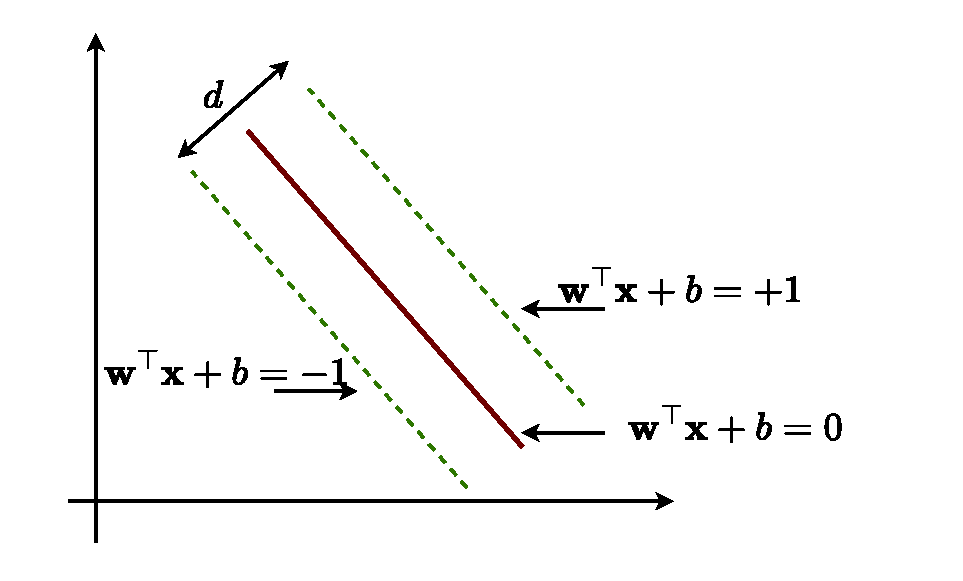
\includegraphics[width=0.99\textwidth]{figures/SVM.pdf}

        \column{0.5\linewidth}
        
A linear support vector machine (SVM) aims to find a decision hyperplane $\wbf^\top \xbf + b = 0$ that maximizes the margin of separation.

\vspace{10pt}

Assume that all data points satisfy the constraints:

\begin{itemize}
    \item $\wbf^\top \xbf_i + b \geq +1$ where $y_i = +1 $
    \item  $\wbf^\top \xbf_i + b \leq -1$ where $y_i = -1 $
\end{itemize}
    \end{columns}

\end{frame}

\begin{frame}{Why $\pm 1$? The Canonical Hyperplane}
    Scaling $(\wbf, b)$ by a constant $c > 0$ leaves the hyperplane $\wbf^\top \xbf + b = 0$ unchanged.

    \vspace{10pt}

    We remove this freedom by fixing the scale so that the closest points satisfy
    \begin{multiequation}
        \min_{i} \; y_i(\wbf^\top \xbf_i + b) = 1
    \end{multiequation}

    The training points then satisfy $y_i(\wbf^\top \xbf_i + b) \geq 1$, and the closest points of the two classes lie on $\wbf^\top \xbf + b = +1$ and $\wbf^\top \xbf + b = -1$.

    \vspace{10pt}

    The two bullet constraints on the previous slide collapse into the single constraint $y_i(\wbf^\top \xbf_i + b) \geq 1$.
\end{frame}


\begin{frame}{The SVM and Linear Classification}
    \begin{center}
    \tikzset{
        leftNode/.style={circle,minimum width=.5ex, fill=Red,draw},
        rightNode/.style={circle,minimum width=.5ex, fill=RoyalBlue,thick,draw},
        rightNodeInLine/.style={solid,circle,minimum width=.7ex, fill=RoyalBlue,thick,draw=white},
        leftNodeInLine/.style={solid,circle,minimum width=.7ex, fill=Red,thick,draw},
    }
    \begin{tikzpicture}[
            scale=1.8,
            important line/.style={thick,color=black}, dashed line/.style={dashed,color=blue},
            every node/.style={color=black},
        ]
        
        \node at (.5,1.55) {\color{Red}\Large$\Rcal_{+}$};
        \node at (3.5,1.55) {\color{RoyalBlue}\Large$\Rcal_{-}$};
        \node at (2.0,2.2) {\color{black}$\x_p$};
        \node at (.5,.5) {\Large$\Hcal$};
        
        \draw[dashed line, yshift=.7cm]
        (.2,.2) coordinate (sls) -- (2.5,2.5) coordinate (sle)
        node[solid,circle,minimum width=2.8ex,fill=none,thick,draw] (name) at (2,2){}
        node[leftNodeInLine] (name) at (2,2){}
        node[solid,circle,minimum width=2.8ex,fill=none,thick,draw] (name) at (1.5,1.5){}
        node[leftNodeInLine] (name) at (1.5,1.5){}
        node [above left,color=Red] {$\wbf^\T \x + b = +1$};

        \draw[important line]
        (.55,.55) coordinate (lines) -- (3,3) coordinate (linee)
        node [above right] {$g(\x) = \wbf^\T \x + b = 0$};

        \draw[dashed line, xshift=.7cm]
        (.2,.2) coordinate (ils) -- (2.5,2.5) coordinate (ile)
        node[solid,circle,minimum width=2.8ex,fill=none,thick,draw] (name) at (1.8,1.8){}
        node[rightNodeInLine] (name) at (1.8,1.8){}
        node [above right,color=RoyalBlue] {$\wbf^\T \x + b = -1$};

        \draw[very thick,<->] ($(sls)+(.2,.2)$) -- ($(ils)+(.2,.2)$)
        node[sloped,above, near end] {Margin};
        
        \draw[very thick,<->] ($(linee)+(-.85,-.85)$) -- ($(ils)+(1.6,1.6)$)
        node[sloped, above, near end] {$r$};
        
        \draw[very thick,<-] ($(sls)+(2.15,2.15)$) -- ($(linee)+(-.3,-.3)$)
        node[sloped, above, near end] {$\wbf$};

        \foreach \Point in {(.9,2.4), (1.3,2.5), (1.3,2.1), (2,3), (1,2.9)}{
        \draw \Point node[leftNode]{};
        }

        \foreach \Point in {(2.9,1.4), (2.3,.5), (3.3,.6), (2,0.9), (2.4,1)}{
        \draw \Point node[rightNode]{};
        }

    \end{tikzpicture}
    \end{center}

\end{frame}

\begin{frame}{Equation for a Hyperplane}

    \begin{columns}
        \column{0.2\linewidth}
        \column{0.3\linewidth}
        $\wbf^\top \xbf = \beta$

        \column{0.5\linewidth}

        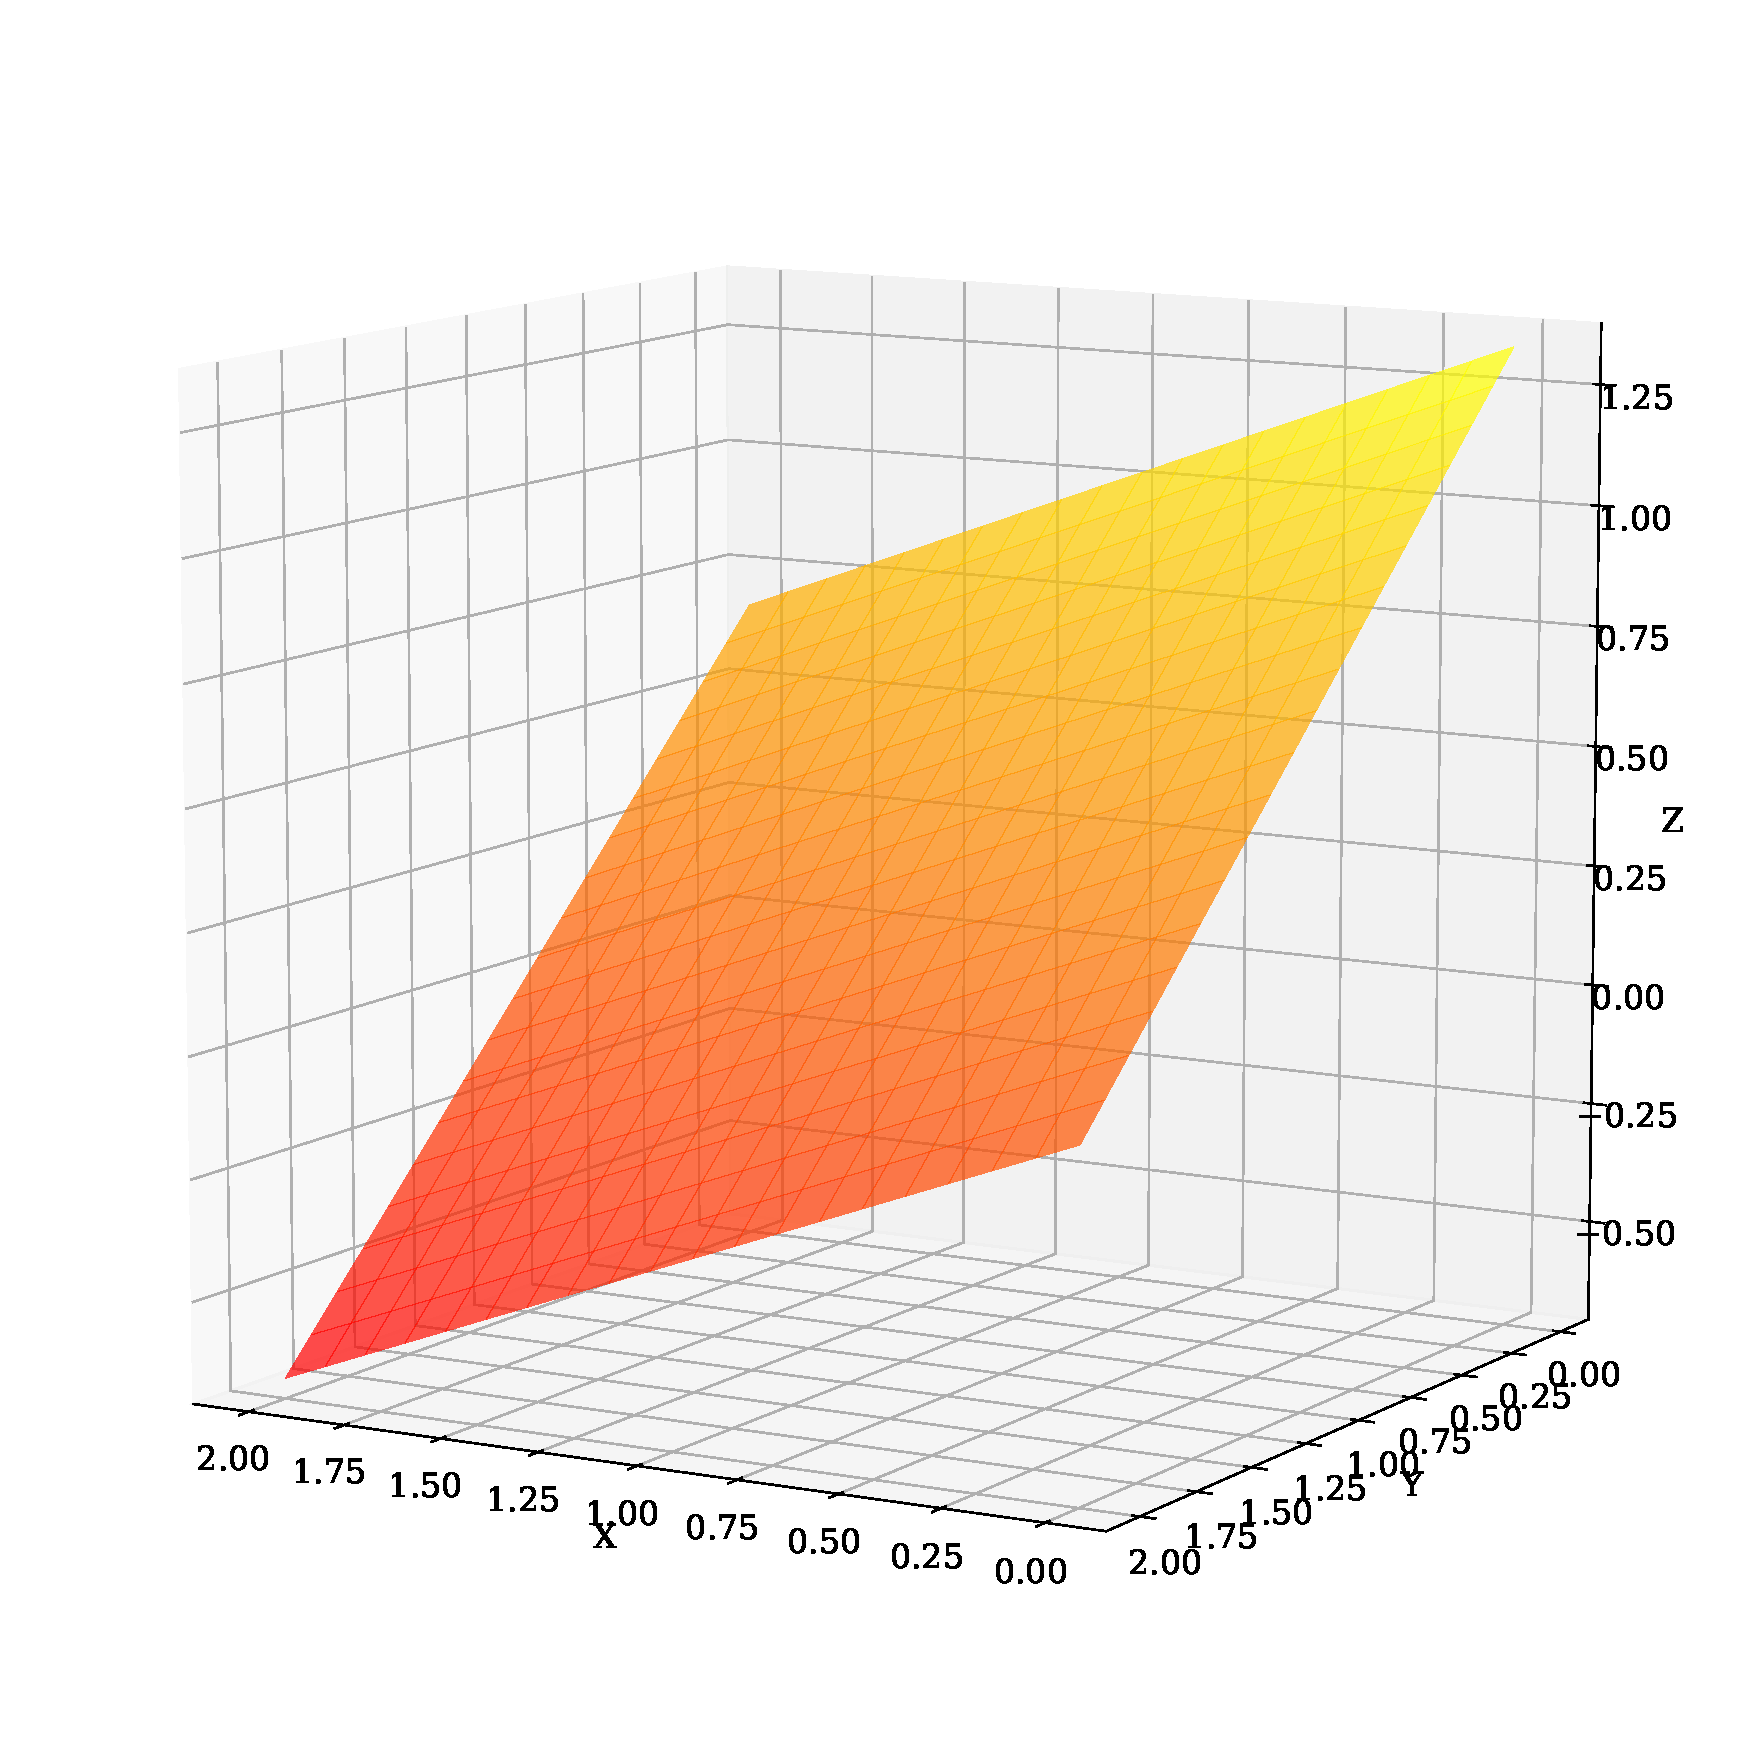
\includegraphics[width=0.80\textwidth]{figures/hyperplane.pdf}


    \end{columns}

\end{frame}

\begin{frame}{Euclidean Projection of a Point on a Hyperplane}

    \begin{columns}
        \column{0.05\linewidth}
        \column{0.45\linewidth}
        We project a point $\xbf_0$ onto the hyperplane  $\wbf^\top \xbf = \beta$.

        The projection point $\xbf^*$ on the hyperplane is given by

        \begin{multiequation}
            \xbf^* =  \xbf_0 + (\beta - \wbf^\top \xbf_0)\cfrac{\wbf}{||\wbf||^2}
        \end{multiequation}

        \column{0.5\linewidth}

        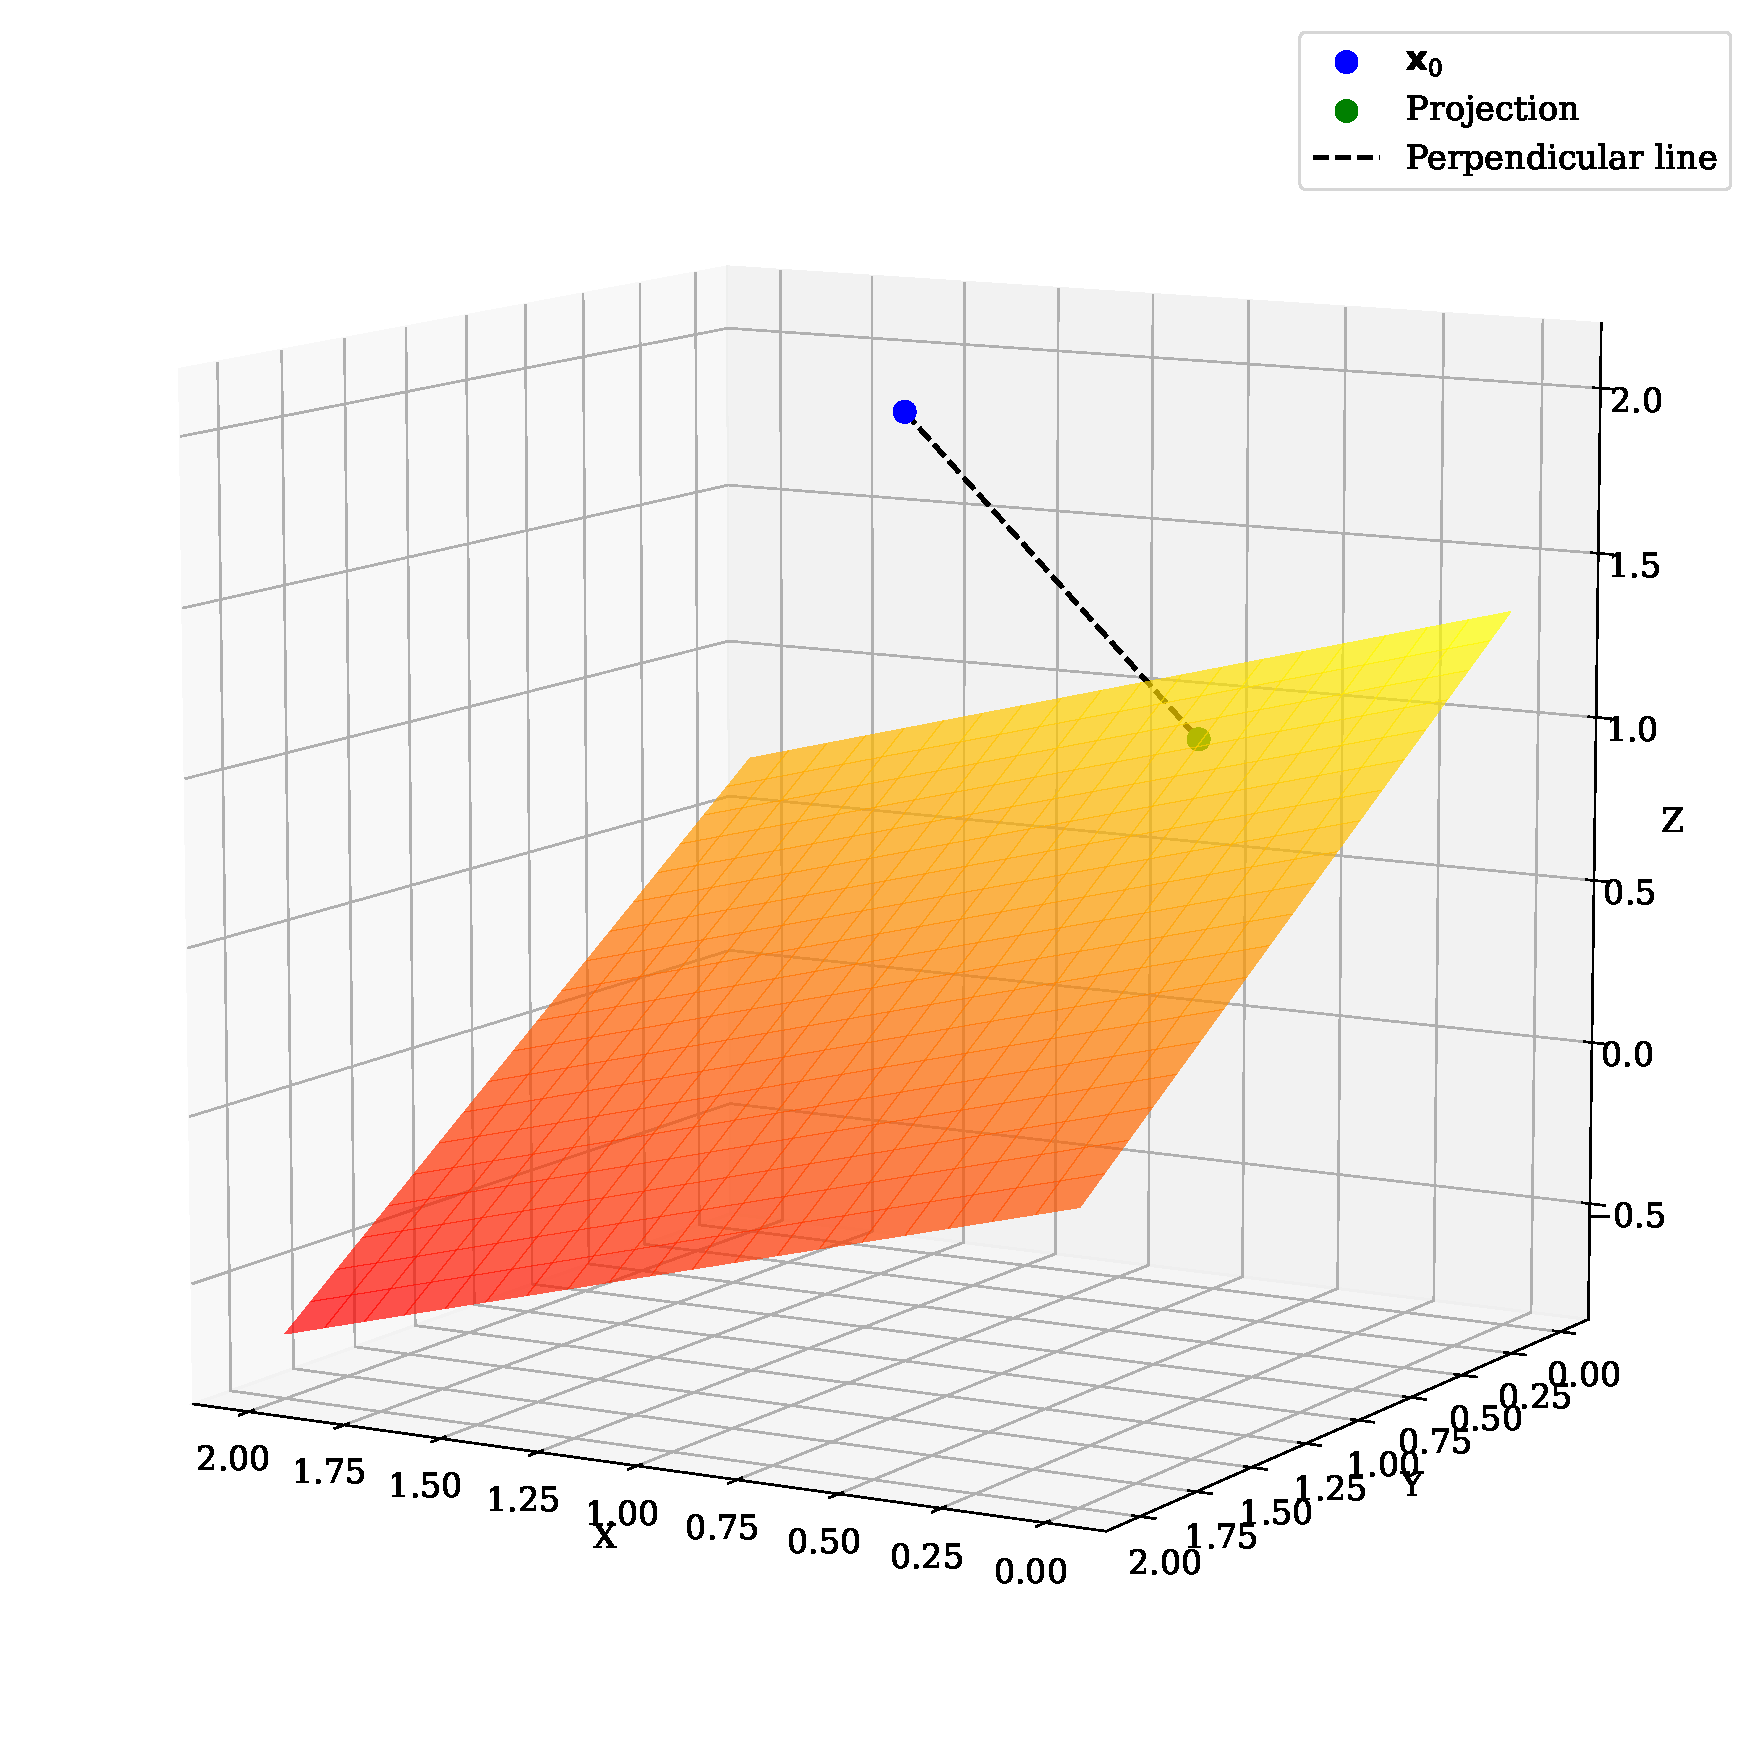
\includegraphics[width=0.80\textwidth]{figures/hyperplane_projection.pdf}


    \end{columns}


\end{frame}

\begin{frame}{Euclidean Projection as an Optimization Problem}

    \begin{columns}
        \column{0.10\linewidth}
        \column{0.65\linewidth}
        One way to derive the above equation is to solve

        $$
            \min_{\xbf} \cfrac{1}{2}||\xbf - \xbf_0||^2
        $$
    
        subject to 
    
        $$
            \wbf^\top \xbf = \beta
        $$

        \column{0.10\linewidth}

    \end{columns}


    
\end{frame}


\begin{frame}{Solving the Projection with a Lagrange Multiplier}
    \begin{multiequation}
        \Lcal(\xbf, \lambda) & = \frac{1}{2}\|\xbf - \xbf_0\|^2 + \lambda(\wbf^\top \xbf - \beta)\\
        \frac{\partial \Lcal}{\partial \xbf} & = \xbf - \xbf_0 + \lambda \wbf = 0 \;\Rightarrow\; \xbf = \xbf_0 - \lambda \wbf\\
        \wbf^\top(\xbf_0 - \lambda\wbf) & = \beta \;\Rightarrow\; \lambda = \frac{\wbf^\top\xbf_0 - \beta}{\|\wbf\|^2}\\
        \xbf^* & = \xbf_0 + (\beta - \wbf^\top\xbf_0)\frac{\wbf}{\|\wbf\|^2}
    \end{multiequation}
    The distance from $\xbf_0$ to the hyperplane is
    \begin{multiequation}
        \|\xbf^* - \xbf_0\| = \frac{|\wbf^\top\xbf_0 - \beta|}{\|\wbf\|}
    \end{multiequation}
    With $\beta = -b$, this is $r = |g(\xbf_0)|/\|\wbf\|$, the distance $r$ in the SVM figure.
\end{frame}

\begin{frame}{Distance between two Hyperplanes}

    \begin{columns}
        \column{0.10\linewidth}
        \column{0.65\linewidth}
       
        Consider two parallel hyperplanes:
        
        $\Hcal_1: \wbf^\top \xbf = b_1$ 

        $\Hcal_2: \wbf^\top \xbf = b_2$

        We compute the distance between them by projecting a point $\xbf_1$ on $\Hcal_1$ onto $\Hcal_2$.

        \begin{multiequation}
            \xbf_2 & =  \xbf_1 + (b_2 - \wbf^\top \xbf_1)\cfrac{\wbf}{||\wbf||^2}\\
            \xbf_2 & =  \xbf_1 + (b_2 - b_1)\cfrac{\wbf}{||\wbf||^2} \quad (\text{since } \wbf^\top \xbf_1 = b_1)
        \end{multiequation}

        \column{0.10\linewidth}

    \end{columns}


\end{frame}

\begin{frame}{Distance between two Hyperplanes}

    \begin{columns}
        \column{0.10\linewidth}
        \column{0.65\linewidth}
    
        Hence, the distance between two hyperplanes is given by 

        \begin{multiequation}
        d = ||\xbf_2 -  \xbf_1|| & = \bigg| \bigg| (b_2 - b_1)\cfrac{\wbf}{||\wbf||^2}\bigg| \bigg|\\
        d = ||\xbf_2 -  \xbf_1|| & = \cfrac{|b_2 - b_1|}{|| \wbf||}
        \end{multiequation}


        \column{0.10\linewidth}

    \end{columns}


\end{frame}



\begin{frame}{Formulating SVM Problem: Hyperplane Distance}

    \begin{columns}
        \column{0.40\linewidth}

    In the SVM problem, the two margin hyperplanes are

    \begin{itemize}
        \item $\wbf^\top \xbf + b = +1$
        \item  $\wbf^\top \xbf + b = -1$ 
    \end{itemize}

    Let $b_1 = 1- b$ and $b_2 = - 1- b$. 


    \column{0.40\linewidth}

    Then, 

    \begin{multiequation}
        d& = || \xbf_2 - \xbf_1 || = \cfrac{|b_2 - b_1|}{|| \wbf||} \\
        & = \cfrac{|- 1- b - 1 + b|}{|| \wbf||} = \cfrac{2}{||\wbf||}
    \end{multiequation}
\end{columns}

\end{frame}

\begin{frame}{Formulating SVM Problem: Objective}

    \begin{columns}
        \column{0.10\linewidth}
        \column{0.65\linewidth}
    
We want to maximize $d$, which is equivalent to minimizing $\cfrac{||\wbf||}{2}$. 


\vspace{20pt}

Both $||\wbf||$ and $\cfrac{||\wbf||^2}{2}$ are convex, and they share the same minimizer. We minimize $\cfrac{||\wbf||^2}{2}$ because it is differentiable everywhere (its gradient is $\wbf$) and turns the problem into a quadratic program.

        \column{0.10\linewidth}

    \end{columns}

\end{frame}


\begin{frame}{Final Optimization Problem for SVM}

    \begin{tblock}{}
        Our discussion of constrained optimization used minimization. The SVM goal of maximizing $d = 2/||\wbf||$ becomes the following minimization:
        \begin{multiequation}
        \wbf^*, b^* = \arg&\min_{\wbf,\, b}  \frac{1}{2}\|\mathbf{w}\|_2^2 \nonumber \\
        & \text{s.t. } y_i (\mathbf{w}^T\mathbf{x}_i+b) \geq 1, \;\; i = 1,\dots,n 
        \hspace{1em}
        {\color{MediumRed}\text{\% } 1 - y_i (\mathbf{w}^T\mathbf{x}_i+b)\leq 0}
        \end{multiequation}
        
        \end{tblock}

\end{frame}

\begin{frame}{Lagrangian for SVM }

    \begin{tblock}{The Lagrangian function for SVM is given by}
        \begin{multiequation}
        \Lcal(\wbf, b, \alpha) =   \frac{1}{2}\|\mathbf{w}\|_2^2 - \sum_{i=1}^{n} \alpha_i\left[ y_i (\mathbf{w}^T\mathbf{x}_i+b) - 1 \right]
        \end{multiequation}
        where $\alpha_i \geq 0$ are the Lagrange multipliers.
        \end{tblock}

\end{frame}


\begin{frame}{From the Primal to the Dual Problem}
    \begin{itemize}
        \item \textbf{Primal:} $\displaystyle \min_{\wbf, b} \; \max_{\alpha \geq 0} \; \Lcal(\wbf, b, \alpha)$.
        The inner maximum is $+\infty$ when a constraint is violated and $\frac{1}{2}\|\wbf\|^2$ otherwise, so this is the original problem.
        \item<2-> \textbf{Dual:} swap the order, $\displaystyle \max_{\alpha \geq 0} \; \min_{\wbf, b} \; \Lcal(\wbf, b, \alpha)$.
        The inner minimum is what we compute next, from $\partial\Lcal/\partial\wbf = 0$ and $\partial\Lcal/\partial b = 0$.
        \item<3-> \textbf{Weak duality:} dual optimum $\leq$ primal optimum.
        \item<4-> \textbf{Strong duality:} the SVM primal is a convex QP with affine constraints, so the two optima are equal when the data are separable. Solving the dual for $\alpha^*$ therefore gives the primal solution $\wbf^*$.
    \end{itemize}
\end{frame}

%------------------------------------------------
\begin{frame}{Deriving the Support Vector Machine}
    \begin{tblock}{}
    
    For fixed $\alpha$, we find the $\wbf$ and $b$ that minimize $\Lcal$. Setting the derivative of $\Lcal$ w.r.t. $\wbf$ equal to zero gives
    \begin{multiequation}
    \frac{\partial \Lcal}{\partial \wbf}  = \wbf - \sum_{i=1}^{n} \alpha_i y_i \mathbf{x}_i = 0  \hspace{1em} \rightarrow \hspace{1em} 
    \wbf = \sum_{i=1}^{n} \alpha_i y_i \mathbf{x}_i \nonumber
    \end{multiequation}
    
    \end{tblock}
    
\end{frame}


%------------------------------------------------
\begin{frame}{Deriving the Support Vector Machine}


    \begin{tblock}{}
    Setting the gradient equal to zero gave us an expression for $\wbf$! Next, we set the derivative of $\Lcal$ w.r.t. $b$ to zero:
    \begin{multiequation}
    \frac{\partial \Lcal}{\partial b}  = -\sum_{i=1}^{n} \alpha_i y_i = 0 \hspace{1em} \rightarrow \hspace{1em} \sum_{i=1}^{n} \alpha_i y_i = 0
    \nonumber
    \end{multiequation}
    {\color{MediumRed}\bf Observation}: By taking the derivative w.r.t. $b$, we ended up getting a constraint! 
    \end{tblock}
    
\end{frame}
    
    
    %------------------------------------------------
    \begin{frame}{Deriving the Support Vector Machine}
    \begin{tblock}{}
    We simplify $\Lcal$ by substituting the expression for $\wbf$ and the constraint $\alpha^\T\ybf = \sum_i \alpha_i y_i = 0$.
    \begin{multiequation}
    \Lcal(\alpha) &=   
    \uncover<2->{
    \frac{1}{2} \sum_{j=1}^{n}\sum_{i=1}^{n} \alpha_i\alpha_j y_i y_j \mathbf{x}_i^\T \mathbf{x}_j   - \sum_{i=1}^{n} \alpha_i  y_i \mathbf{w}^\T\mathbf{x}_i - b \sum_{i=1}^{n} \alpha_i y_i  + \sum_{i=1}^{n} \alpha_i \nonumber  }\\
    \uncover<3->{
    &=\frac{1}{2} \sum_{j=1}^{n}\sum_{i=1}^{n} \alpha_i\alpha_j y_i y_j \mathbf{x}_i^\T \mathbf{x}_j   - \sum_{i=1}^{n} \sum_{j=1}^{n}\alpha_i \alpha_j  y_i y_j \xbf_i^\T\mathbf{x}_j  + \sum_{i=1}^{n} \alpha_i  \nonumber}  \\
    \uncover<4->{
    &= \sum_{i=1}^{n} \alpha_i - \frac{1}{2}   \sum_{j=1}^{n}\sum_{i=1}^{n} \alpha_i\alpha_j y_i y_j \mathbf{x}_i^\T \mathbf{x}_j \nonumber}
    \end{multiequation}
    \end{tblock}
    \end{frame}
    
    
    
    %------------------------------------------------
    \begin{frame}{Summary of the SVM so far}
    \begin{itemize}
    \item The expression below is known as the {\em dual form} of the constrained optimization task, which is maximized over $\alpha$. Note that $\mathbf{x}_i^\T \mathbf{x}_j$ measures the similarity between two vectors, so we can replace it with a kernel function $\kappa(\mathbf{x}_i, \mathbf{x}_j )$.
    \begin{multiequation}
    \arg\max_{\alpha}
    \sum_{i=1}^{n} \alpha_i - \frac{1}{2}   \sum_{j=1}^{n}\sum_{i=1}^{n} \alpha_i\alpha_j y_i y_j \kappa(\mathbf{x}_i, \mathbf{x}_j ), 
    \text{ s.t. }
    \sum_{i=1}^n y_i\alpha_i = 0, \alpha_i \geq 0
    \end{multiequation}
    \item<2-> Let $\Phi(\x)$ be a high-dimensional nonlinear representation of $\x$. 
    \uncover<2->{
    \begin{multiequation}
    \wbf^\T\Phi(\x) + b = \left( \sum_{i=1}^n \alpha_i y_i \Phi(\xbf_i) \right)^\T \Phi(\xbf) + b
    =  \sum_{i=1}^n \alpha_i y_i \Phi(\xbf_i)^\T \Phi(\xbf) + b
    \end{multiequation}
    where $\kappa(\mathbf{x}_i, \mathbf{x}_j ) = \Phi(\xbf_i)^\T \Phi(\xbf_j) $. The data enter these expressions only through dot products.
    }
    \end{itemize}
    \end{frame}
    
    
    \begin{frame}{Support Vectors from the KKT Conditions}
    Complementary slackness for the SVM constraints gives
    \begin{multiequation}
        \alpha_i^* \left[ y_i(\wbf^{*\top}\xbf_i + b^*) - 1 \right] = 0, \quad i = 1, \dots, n
    \end{multiequation}
    \begin{itemize}
        \item If $y_i(\wbf^{*\top}\xbf_i + b^*) > 1$, the point lies beyond the margin, so $\alpha_i^* = 0$.
        \item<2-> If $\alpha_i^* > 0$, then $y_i(\wbf^{*\top}\xbf_i + b^*) = 1$, and the point lies on the margin. These points are the {\color{MediumRed}\textbf{support vectors}}.
    \end{itemize}
    \uncover<3->{
    Since $\wbf^* = \sum_i \alpha_i^* y_i \xbf_i$, only the support vectors determine the hyperplane. Removing a non-support vector from the training set leaves the solution unchanged.
    }
\end{frame}



%------------------------------------------------
\begin{frame}{Recovering $b$ and Classifying a New Point}
    Pick a support vector $\xbf_s$ with $\alpha_s^* > 0$. From $y_s(\wbf^{*\top}\xbf_s + b^*) = 1$ and $y_s^2 = 1$:
    \begin{multiequation}
        b^* = y_s - \sum_{i \in \mathcal{S}} \alpha_i^* y_i \, \kappa(\xbf_i, \xbf_s)
    \end{multiequation}
    where $\mathcal{S}$ is the set of support vectors. In practice, average $b^*$ over the support vectors for numerical stability (for the soft margin, use those with $0 < \alpha_s^* < C$).

    \vspace{8pt}

    \textbf{Decision rule} for a new point $\xbf$:
    \begin{multiequation}
        \hat{y} = \operatorname{sign}\left( \sum_{i \in \mathcal{S}} \alpha_i^* y_i \, \kappa(\xbf_i, \xbf) + b^* \right)
    \end{multiequation}
    Prediction cost grows with the number of support vectors $|\mathcal{S}|$, which is usually much smaller than $n$.
\end{frame}


%------------------------------------------------
% Worked example. Verified with sklearn SVC(kernel='linear', C=1e8):
% coef_ = [1, 0], intercept_ = -1, dual_coef_ = [-0.5, 0.5], support_ = [2, 1].
%------------------------------------------------
\begin{frame}{Worked Example: Hard Margin SVM by Hand}
    \begin{columns}
    \column{0.40\linewidth}
    Data:
    \begin{itemize}
        \item $\xbf_1 = (3, 2)$, \; $y_1 = +1$
        \item $\xbf_2 = (2, 0)$, \; $y_2 = +1$
        \item $\xbf_3 = (0, 0)$, \; $y_3 = -1$
    \end{itemize}

    \vspace{6pt}

    Guess from a sketch: $\xbf_2$ and $\xbf_3$ are the support vectors, so $\alpha_1 = 0$.

    \vspace{6pt}

    $\sum_i \alpha_i y_i = 0 \;\Rightarrow\; \alpha_2 = \alpha_3 = \alpha$.

    \column{0.56\linewidth}
    \uncover<2->{
    \begin{multiequation}
        \Lcal(\alpha) & = 2\alpha - \frac{1}{2}\alpha^2 \, \|\xbf_2 - \xbf_3\|^2 = 2\alpha - 2\alpha^2\\
        \frac{d\Lcal}{d\alpha} & = 2 - 4\alpha = 0 \;\Rightarrow\; \alpha = \tfrac{1}{2}\\
        \wbf^* & = \tfrac{1}{2}\xbf_2 - \tfrac{1}{2}\xbf_3 = (1, 0)\\
        b^* & = y_2 - \wbf^{*\top}\xbf_2 = 1 - 2 = -1
    \end{multiequation}
    }
    \uncover<3->{
    Boundary: the vertical line through $(1, 0)$. Margin: $2/\|\wbf^*\| = 2$.

    \vspace{4pt}

    Check $\xbf_1$: $y_1(\wbf^{*\top}\xbf_1 + b^*) = 2 > 1$, so $\alpha_1 = 0$ agrees with the KKT conditions.
    }
    \end{columns}
\end{frame}


%%%%%%%%%%%%%%%%%%%%%%%%%%%%%%%%%%%%%%%%%%%%%%%%%%%%%
\begin{sectionframe}{\faDeviantart}{Nonlinear Support Vector Machine and Kernel}
\end{sectionframe}


\begin{frame}{Nonlinearly Separable Data}

    \Large
    

    \begin{center}
        Most real-world problems exhibit data that are not linearly separable.

    \end{center}

\end{frame}

\begin{frame}{Nonlinearly Separable Data}


    \begin{center}

        How do we separate these two classes?

        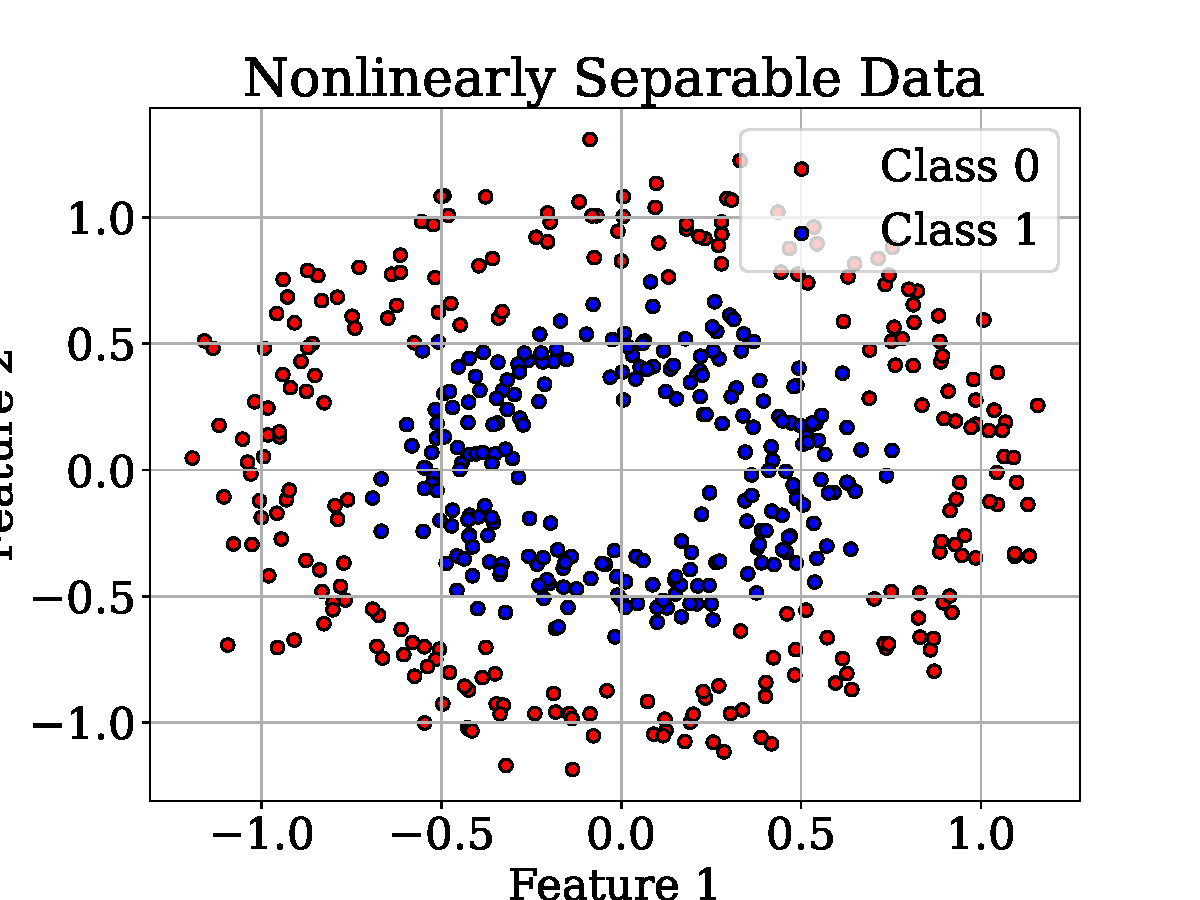
\includegraphics[width=0.49\textwidth]{figures/nonlinearly_separable_data.pdf}
        
    \end{center}

\end{frame}

\begin{frame}{Kernel for Nonlinear Separation}
    
Solution: map the original features into a higher-dimensional space with a function $\Phi(\xbf)$, called the \textbf{feature map}. A \textbf{kernel} computes the dot product in that space directly: $\kappa(\xbf, \xbf') = \Phi(\xbf)^\T \Phi(\xbf')$.

\end{frame}


%------------------------------------------------
\begin{frame}{What are kernels?}

    {\bf\color{MediumRed}In layman's terms}: \uncover<2->{A kernel is a measure of similarity between two 
    patterns $\mathbf{x}$ and $\mathbf{x}'$}
    \begin{itemize}
        
        \item<3-> Consider a similarity measure of the form:
            \begin{multiequation}
            \kappa: & \mathcal{X}\times\mathcal{X}\rightarrow\mathbb{R}\nonumber\\
                & (\mathbf{x},\mathbf{x}')\mapsto \kappa(\mathbf{x},\mathbf{x}')
            \end{multiequation}

        \begin{itemize}
            \item<4-> $\kappa(\mathbf{x},\mathbf{x}')$ returns a real-valued quantity measuring the similarity 
                between $\mathbf{x}$ and $\mathbf{x}'$
            \item<5-> One simple measure of similarity is the {\textrm{\em canonical dot product}}
                \begin{itemize}
                \item<5-> computes the cosine of the angle between two vectors, provided they are normalized
                    to length 1
                \item<5-> a vector space equipped with a dot product is a {\textrm{\em pre-Hilbert space}} (inner product space)
                \end{itemize}
            \end{itemize}
            
        \item<6-> A feature map $\Phi$ {\bf\color{MediumRed}represents} patterns in a dot product space $\mathcal{H}$, where the kernel computes dot products \uncover<6->{
            \begin{multiequation}
            \Phi: \mathcal{X}\rightarrow\mathcal{H}
            \end{multiequation}
        } 
        
    \end{itemize}
\end{frame}

%------------------------------------------------
\begin{frame}{Feature Space: $\mathcal{X}\rightarrow\mathcal{H}$}

    \begin{tblock}{}
    A few notes about our mapping into $\mathcal{H}$ via $\Phi$
        \begin{enumerate}
        \item Mapping lets us define a similarity measure from the dot product in $\mathcal{H}$
            \begin{multiequation}
            \kappa(\mathbf{x},\mathbf{x}'):=\Phi(\mathbf{x})^\T\Phi(\mathbf{x}')
            \end{multiequation}
        \item<2-> Patterns are dealt with geometrically; efficient learning algorithms may be 
            applied using linear algebra
        \item<3-> Different choices of $\Phi(\cdot)$ give different similarity measures
        \end{enumerate}
    \end{tblock}
\end{frame}

\begin{frame}{A simple kernel example}

    Consider the dot product of two mapped vectors $\mathbf{x}, \mathbf{z} \in \mathbb{R}^2$:
    \begin{multiequation}
    \Phi(\mathbf{x})^\T\Phi(\mathbf{z}) =
    \begin{bmatrix}
        x_1^2 \\
        \sqrt{2}x_1 x_2 \\
        x_2^2
    \end{bmatrix}^\T
    \begin{bmatrix}
        z_1^2 \\
        \sqrt{2}z_1 z_2 \\
        z_2^2
    \end{bmatrix}
    = x_1^2z_1^2 + 2 x_1x_2z_1z_2 + x_2^2z_2^2 \\
    = (x_1z_1 + x_2z_2)^2
    = (\mathbf{x}^\T\mathbf{z})^2 = \kappa(\mathbf{x},\mathbf{z})
    \end{multiequation}

\end{frame}

%------------------------------------------------
\begin{frame}{A simple kernel example}
\begin{center}
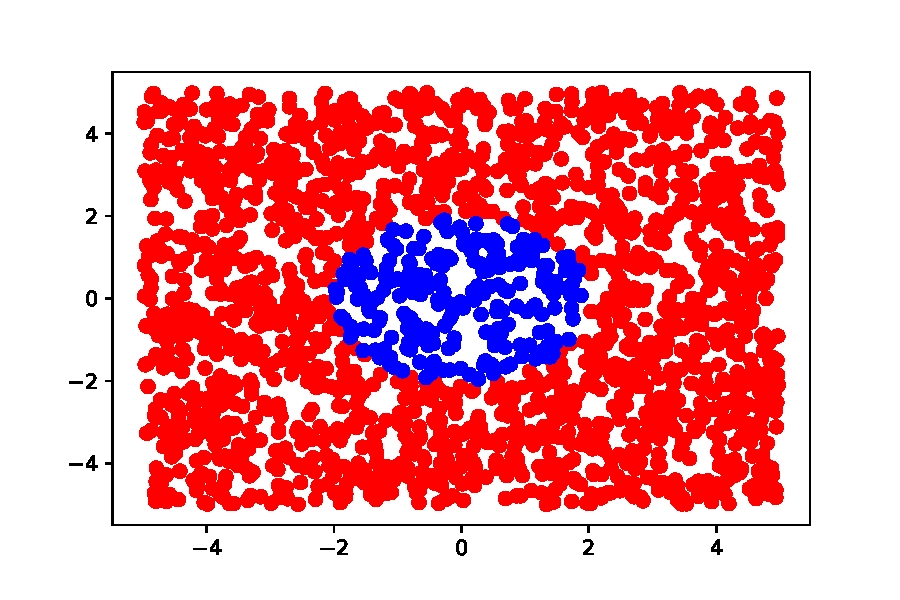
\includegraphics[width=.47\textwidth]{figures/svm-2d-example.pdf}
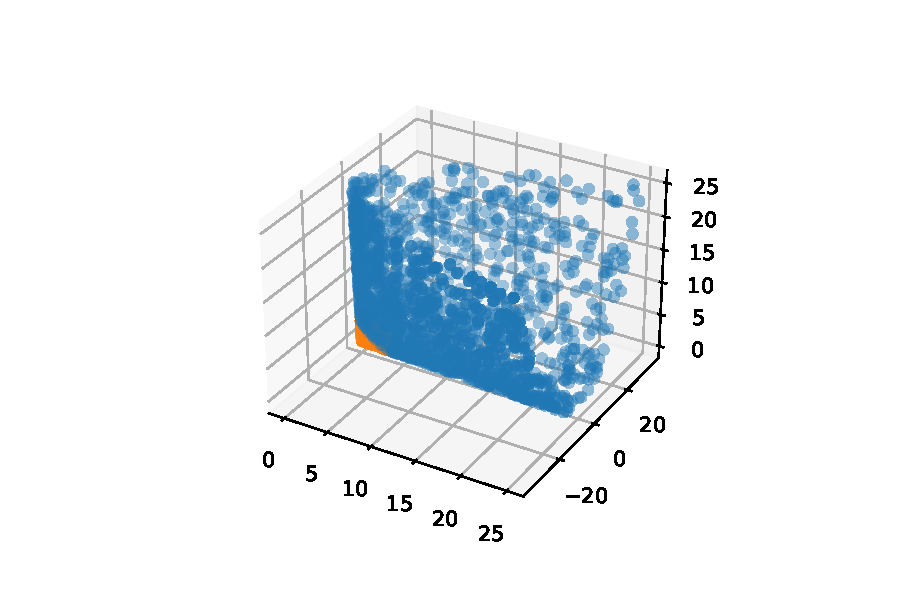
\includegraphics[width=.47\textwidth]{figures/svm-3d-example.pdf}
\end{center}
\end{frame}


%------------------------------------------------
\begin{frame}{Gaussian Kernel}
    \small 
\begin{tblock}{}
    The Gaussian kernel is defined as
\begin{multiequation}
        \kappa(\mathbf{x},\mathbf{x}')=\exp{\left(-\gamma\|\mathbf{x}-\mathbf{x}'\|^2\right)}
\end{multiequation}

The term in the exponent ($-\gamma\|\mathbf{x}-\mathbf{x}'\|^2$) is a scalar 
value computed in the vector space of the data. Recall the dot product 
    for two arbitrary vectors is given by
    \begin{multiequation}
        \mathbf{x}^T\mathbf{x}'=\sum\limits_{i=1}^{d}{x_i x_i'}
    \end{multiequation}
    
    Expanding $\|\mathbf{x}-\mathbf{x}'\|^2 = \|\mathbf{x}\|^2 + \|\mathbf{x}'\|^2 - 2\mathbf{x}^\T\mathbf{x}'$ exposes a dot product:
        \begin{multiequation}
        \kappa(\mathbf{x},\mathbf{x}') = e^{-\gamma\|\mathbf{x}\|^2}\, e^{-\gamma\|\mathbf{x}'\|^2}\, e^{2\gamma\mathbf{x}^\T\mathbf{x}'}
            = e^{-\gamma\|\mathbf{x}\|^2}\, e^{-\gamma\|\mathbf{x}'\|^2} \sum\limits_{n=0}^{\infty}\frac{(2\gamma)^n}{n!}\left(\mathbf{x}^\T\mathbf{x}'\right)^n
        \end{multiequation}
    The term $(\mathbf{x}^\T\mathbf{x}')^n$ is a polynomial kernel with a finite feature map. The infinite sum therefore corresponds to an infinite-dimensional $\Phi$.
    
\end{tblock}

\end{frame}



%------------------------------------------------
\begin{frame}{The Kernel Trick}
\begin{itemize}
\item The ``trick'' in each of the kernel examples is that we never needed to calculate $\Phi(\x)$. Instead, we applied a nonlinear function to a dot product and this was equivalent to the dot product in a high dimensional space. 
\begin{itemize}
    \item {\em This is known as the kernel trick!}
    \item Kernels allow us to solve nonlinear classification problems by taking advantage of Cover's Theorem without the overhead of finding the high dimensional space. 
\end{itemize}
\end{itemize}
\end{frame}


\begin{frame}{Cover's Theorem}
    \begin{tblock}{Cover (1965)}
    A pattern classification problem cast nonlinearly into a high-dimensional space is more likely to be linearly separable than in a low-dimensional space.
    \end{tblock}
    \begin{itemize}
        \item For $n$ points in general position in $\mathbb{R}^d$, the fraction of the $2^n$ labelings that a hyperplane can separate is
        \begin{multiequation}
            P(n, d) = \frac{1}{2^{n-1}} \sum_{m=0}^{d} \binom{n-1}{m}
        \end{multiequation}
        \item $P(n, d) = 1$ when $n \leq d + 1$. Example: $P(4, 2) = 7/8$, since XOR cannot be separated in $\mathbb{R}^2$.
        \item Raising $d$ through $\Phi$ raises the chance of separability. The kernel trick gives us that space without computing $\Phi$.
    \end{itemize}
\end{frame}

%------------------------------------------------
\begin{frame}{Which Functions Are Valid Kernels?}
    \begin{itemize}
        \item $\kappa$ is a valid kernel when a feature map $\Phi$ exists with $\kappa(\xbf, \xbf') = \Phi(\xbf)^\T\Phi(\xbf')$.
        \item<2-> \textbf{Mercer's condition:} $\kappa$ is symmetric, and the Gram matrix $K_{ij} = \kappa(\xbf_i, \xbf_j)$ is positive semidefinite for any finite set of points.
        \item<3-> A PSD Gram matrix keeps the dual a convex QP, so the solver reaches the global optimum.
        \item<4-> Linear, polynomial ($c \geq 0$), and Gaussian kernels satisfy Mercer's condition. The $\tanh$ kernel fails it for some $(\gamma, c)$, so its Gram matrix can have negative eigenvalues.
        \item<5-> Sums and products of valid kernels are valid kernels.
    \end{itemize}
\end{frame}


%------------------------------------------------
\begin{frame}{Other popular kernel choices}

{\bf Radial Basis Function (RBF) Kernel} (the Gaussian kernel)
\begin{multiequation}
\kappa(\mathbf{x},\mathbf{z})=\exp{\left(-\gamma\|\mathbf{x}-\mathbf{z}\|^2\right)}
\end{multiequation}
{\bf Polynomial Kernel}
\begin{multiequation}
\kappa(\mathbf{x},\mathbf{z})= (\gamma\,\mathbf{x}^\T \mathbf{z} + c)^p
\end{multiequation}
{\bf Hyperbolic Tangent Kernel}
\begin{multiequation}
\kappa(\mathbf{x},\mathbf{z})=\tanh(\gamma\,\mathbf{x}^\T \mathbf{z} + c)
\end{multiequation}


\end{frame}


%%%%%%%%%%%%%%%%%%%%%%%%%%%%%%%%%%%%%%%%%%%%%%%%%%%%%
\begin{sectionframe}{\faLowVision}{Soft Margin: Allowing Margin Violations}
\end{sectionframe}


\begin{frame}{Soft Margin for SVM}

    \Large 
    
    Some data sets cannot be separated by a linear hyperplane because of outliers, noise, or weak nonlinearity. To keep a linear boundary, we let some points violate the margin or be misclassified, at a cost.

\end{frame}

\begin{frame}{Slack Variable}

    \Large 
    We introduce a slack variable $\xi_i \geq 0$ for sample $i$ such that

    $$
y_i (\wbf^\top \xbf_i  + b) \geq 1 - \xi_i
    $$
\end{frame}



\begin{frame}{Soft Margin Optimization Problem}

    \begin{tblock}{A New Formulation}
        We can modify the objective of maximizing the margin by introducing {\em slack variables} to meet the constraints  
        \begin{multiequation}
        \arg\min_{\wbf, b, \xi} &\frac{1}{2}\|\wbf\|_2^2 + C\sum_{i=1}^{n}\xi_i,\\
        \textrm{s.t. }& y_i(\wbf^T\x_i+b) \geqslant 1 - \xi_i, \quad \xi_i \geqslant 0
        \end{multiequation}
        where $\xi_i > 0$ only for samples that violate the margin, and $C > 0$ sets the price of a violation (large $C$ approaches the hard margin).
        \end{tblock}

\end{frame}


%------------------------------------------------
\begin{frame}{Deriving the Soft Margin SVM}

    
    \begin{tblock}{}
    The Lagrangian function is given by
    \begin{multiequation}
    L(\wbf, b, \xi, \alpha, \mu) = 
    \frac{1}{2}\|\mathbf{w}\|_2^2 
    + C\sum_{i=1}^{n}\xi_i
    - \sum_{i=1}^n \mu_i \xi_i
    - \sum_{i=1}^{n} \alpha_i\left[ y_i (\mathbf{w}^T\mathbf{x}_i+b) - 1 + \xi_i \right]
    \end{multiequation}
    where $\alpha_i \geq 0$ and $\mu_i \geq 0$ are Lagrange multipliers.
    \end{tblock}
    
    
    \uncover<2->{
    \begin{tblock}{}
    Our approach is the same as it was with the hard margin SVM. We have the Lagrangian function and we're going to find the dual form by computing
    \begin{multiequation}
    \frac{\partial L}{\partial \wbf}, \hspace{1em}
    \frac{\partial L}{\partial b}, \hspace{1em}
    \frac{\partial L}{\partial \xi_i}
    \end{multiequation}
    \end{tblock}
    }
    \end{frame}
    
    
    
    
    %------------------------------------------------
    \begin{frame}{Deriving the Soft Margin SVM}
    
    \begin{tblock}{}
    \begin{multiequation}
    \frac{\partial L}{\partial \wbf} = \wbf - \sum_{i=1}^n \alpha_i y_i \xbf_i = 0  \longrightarrow \wbf = \sum_{i=1}^n \alpha_i y_i \xbf_i 
    \hspace{1em}
    {\color{MediumRed}\text{\% same result as before}}
    \end{multiequation}
    \end{tblock}
    
    \uncover<2->{
    \begin{tblock}{}
    \begin{multiequation}
    \frac{\partial L}{\partial \xi_i} = C - \alpha_i - \mu_i = 0 
     \longrightarrow C =  \alpha_i + \mu_i
    \hspace{1em}
    {\color{MediumRed}\text{\% } 0 \leq \alpha_i \leq C \text{ since } \mu_i \geq 0}
    \end{multiequation}
    \end{tblock}
    }
    
    \uncover<3->{
    \begin{tblock}{}
    \begin{multiequation}
    \frac{\partial L}{\partial b} = -\sum_{i=1}^n \alpha_i y_i = 0  
    \longrightarrow \sum_{i=1}^n \alpha_i y_i = 0  
    \hspace{1em}
    {\color{MediumRed}\text{\% same result as before}}
    \end{multiequation}
    \end{tblock}
    }
    
    Substitute these results back into $L$. The $\xi_i$ terms cancel because $\alpha_i + \mu_i = C$.
    
    \end{frame}
    
    
    
    %------------------------------------------------
    \begin{frame}{Deriving the Soft Margin SVM}
    
    \begin{tblock}{}
    \begin{multiequation}
    L(\alpha) &= \uncover<2->{
    \sum_{i=1}^n \alpha_i
    - \frac{1}{2}\sum_{i=1}^n\sum_{j=1}^n \alpha_i\alpha_j y_i y_j \x_i^\T \x_j
    +C\sum_{i=1}^n \xi_i 
    -\sum_{i=1}^n\alpha_i\xi_i
    -\sum_{i=1}^n\mu_i\xi_i} \\
    \uncover<3->{
    &=
    \sum_{i=1}^n \alpha_i
    - \frac{1}{2}\sum_{i=1}^n\sum_{j=1}^n \alpha_i\alpha_j y_i y_j \x_i^\T \x_j
    +C\sum_{i=1}^n \xi_i 
    - \sum_{i=1}^n \xi_i (\alpha_i + \mu_i) }\\
    \uncover<4->{
    &=
    \sum_{i=1}^n \alpha_i
    - \frac{1}{2}\sum_{i=1}^n\sum_{j=1}^n \alpha_i\alpha_j y_i y_j \x_i^\T \x_j
    +C\sum_{i=1}^n \xi_i 
    -C\sum_{i=1}^n \xi_i}\\
    \uncover<5->{
    &=
    \sum_{i=1}^n \alpha_i
    - \frac{1}{2}\sum_{i=1}^n\sum_{j=1}^n \alpha_i\alpha_j y_i y_j \x_i^\T \x_j
    \hspace{1em}
    {\color{MediumRed}\text{\% same result as the hard margin}}
    }
    \end{multiequation}
    \end{tblock}
    
    \end{frame}
    
    
    
    %------------------------------------------------
    \begin{frame}{The Soft Margin SVM}
    \begin{tblock}{}
    
    \begin{multiequation}
    \arg\max_{\alpha}
    \sum_{i=1}^{n} \alpha_i - \frac{1}{2}   \sum_{j=1}^{n}\sum_{i=1}^{n} \alpha_i\alpha_j y_i y_j \kappa(\mathbf{x}_i, \mathbf{x}_j ), 
    \text{ s.t. }
    \sum_{i=1}^n y_i\alpha_i = 0, 0 \leq \alpha_i \leq C
    \end{multiequation}
    \end{tblock}
    
    \begin{itemize}
    \item The soft margin dual matches the hard margin dual except for one change: the Lagrange multiplier $\alpha_i$ is now bounded above by $C$ (a \emph{box constraint}).
    \item<2-> The optimization problem might look difficult; however, this is a {\em quadratic program} and there are optimizers available to solve this problem. See \texttt{CVXOPT} or \texttt{CVXPY} in Python. The \texttt{SVC} class in \texttt{scikit-learn} solves it with an SMO-type algorithm (\texttt{libsvm}).
    \item<3-> Many $\alpha_i$ will be zero after solving the QP. The data samples that correspond to non-zero values of $\alpha_i$ are known as the {\em \color{MediumRed} support vectors}. 
    \end{itemize}
    
        
\end{frame}


\begin{frame}{Interpreting $\alpha_i$ and $\xi_i$ in the Soft Margin SVM}
    KKT conditions: $\alpha_i\left[y_i f(\xbf_i) - 1 + \xi_i\right] = 0$ and $\mu_i \xi_i = (C - \alpha_i)\,\xi_i = 0$, with $f(\xbf) = \wbf^\T\xbf + b$.

    \vspace{10pt}

    \begin{center}
    \begin{tabular}{lll}
        \toprule
        $\alpha_i$ & Condition & Location of $\xbf_i$ \\
        \midrule
        $\alpha_i = 0$ & $y_i f(\xbf_i) \geq 1$, \; $\xi_i = 0$ & correct side, on or beyond the margin \\
        $0 < \alpha_i < C$ & $y_i f(\xbf_i) = 1$, \; $\xi_i = 0$ & exactly on the margin \\
        $\alpha_i = C$ & $y_i f(\xbf_i) = 1 - \xi_i$ & inside the margin ($0 < \xi_i \leq 1$) \\
         & & or misclassified ($\xi_i > 1$) \\
        \bottomrule
    \end{tabular}
    \end{center}

    \vspace{6pt}

    Support vectors are the points with $\alpha_i > 0$ (rows 2 and 3).
\end{frame}


%------------------------------------------------
% Connects to LinearSVC(loss="hinge") in the notebook and to logistic regression.
%------------------------------------------------
\begin{frame}{Soft Margin SVM as Hinge Loss Minimization}
    At the optimum, $\xi_i = \max\left(0,\, 1 - y_i(\wbf^\T\xbf_i + b)\right)$. Substituting into the primal:
    \begin{multiequation}
        \min_{\wbf, b} \; \frac{1}{2}\|\wbf\|^2 + C \sum_{i=1}^{n} \underbrace{\max\left(0,\, 1 - y_i(\wbf^\T\xbf_i + b)\right)}_{\text{hinge loss}}
    \end{multiequation}
    \begin{columns}
    \column{0.52\linewidth}
    \begin{itemize}
        \item Regularized loss minimization, the same template as regularized logistic regression with loss $\log(1 + e^{-y f(\xbf)})$.
        \item Hinge loss is exactly zero for $y f(\xbf) \geq 1$, which is why many $\alpha_i$ are zero.
        \item \texttt{LinearSVC(loss="hinge")} in the notebook solves this problem (it also regularizes $b$).
    \end{itemize}
    \column{0.44\linewidth}
    \begin{tikzpicture}
    \begin{axis}[width=\linewidth, height=0.8\linewidth, xlabel={$y f(\xbf)$}, ylabel={loss},
                 domain=-2:3, samples=120, ymin=0, ymax=3.2, axis lines=left,
                 legend style={font=\tiny, draw=none}, tick label style={font=\tiny}, label style={font=\small}]
        \addplot[thick, red] {max(0, 1-x)};
        \addlegendentry{hinge}
        \addplot[thick, blue, dashed] {ln(1+exp(-x))/ln(2)};
        \addlegendentry{logistic (scaled)}
        \addplot[thick, black, dotted] coordinates {(-2,1) (0,1) (0,0) (3,0)};
        \addlegendentry{0-1}
    \end{axis}
    \end{tikzpicture}
    \end{columns}
\end{frame}


%------------------------------------------------
% Figures from ch12_new_figures.py
%------------------------------------------------
\begin{frame}{Effect of $C$ (Linear Kernel)}
    \begin{center}
    \includegraphics[width=0.95\textwidth]{figures/svm_C_effect.pdf}
    \end{center}
    Small $C$ tolerates violations: wide margin, many support vectors. Large $C$ punishes them: narrow margin, close to the hard margin solution.
\end{frame}


%------------------------------------------------
\begin{frame}{Effect of $\gamma$ (RBF Kernel)}
    \begin{center}
    \includegraphics[width=0.95\textwidth]{figures/svm_gamma_effect.pdf}
    \end{center}
    $\gamma$ sets how far the influence of a training point reaches in $\kappa(\xbf, \xbf') = e^{-\gamma\|\xbf - \xbf'\|^2}$. Small $\gamma$ underfits. Large $\gamma$ wraps the boundary around single points: training accuracy rises while test accuracy falls. Tune $C$ and $\gamma$ together with cross-validation.
\end{frame}


%------------------------------------------------
% The notebook classifies 6 modulation types, but the slides never cover multi-class.
%------------------------------------------------
\begin{frame}{Multi-class SVM}
    The SVM is a binary classifier. For $K$ classes:
    \begin{itemize}
        \item \textbf{One-vs-Rest (OvR):} train $K$ classifiers, class $k$ against the rest. Predict the class with the largest $f_k(\xbf)$.
        \item<2-> \textbf{One-vs-One (OvO):} train $K(K-1)/2$ classifiers, one per pair of classes. Predict by majority vote.
        \item<3-> \texttt{SVC} always trains OvO internally. Its \texttt{decision\_function\_shape} argument only changes the shape of the returned scores. \texttt{LinearSVC} uses OvR.
    \end{itemize}
    \uncover<4->{
    Notebook example: $K = 6$ modulation types gives $15$ pairwise SVMs.
    }
\end{frame}


%------------------------------------------------
\begin{frame}{From the Math to \texttt{scikit-learn}}
    \begin{center}
    \small
    \begin{tabular}{ll}
        \toprule
        Math & \texttt{SVC} parameter or attribute \\
        \midrule
        $C$ & \texttt{C} \\
        $\gamma$ in RBF, polynomial, $\tanh$ & \texttt{gamma} \\
        $c$ and $p$ in the polynomial kernel & \texttt{coef0}, \texttt{degree} \\
        support vectors $\{\xbf_i : \alpha_i > 0\}$ & \texttt{support\_vectors\_}, \texttt{support\_} \\
        $\alpha_i y_i$ for the support vectors & \texttt{dual\_coef\_} \\
        $b$ & \texttt{intercept\_} \\
        $\wbf$ (linear kernel only) & \texttt{coef\_} \\
        $\sum_i \alpha_i y_i \kappa(\xbf_i, \xbf) + b$ & \texttt{decision\_function(X)} \\
        \bottomrule
    \end{tabular}
    \end{center}
    Kernels depend on distances and dot products, so standardize features first (\texttt{StandardScaler}). Training cost grows roughly as $n^2$ or faster, so use \texttt{LinearSVC} or \texttt{SGDClassifier} for large $n$.
\end{frame}


    
    
\begin{frame}{References}
    % Beamer does not support BibTeX so references must be inserted manually as below
    \footnotesize{
        \begin{thebibliography}{99}
            \bibitem[Bishop, 2007]{p1} Christopher Bishop (2007)
            \newblock Pattern Recognition and Machine Learning
            \newblock \emph{New York, NY: Springer} 1st edition.
            \bibitem[Vapnik, 2000]{p2} Vladimir Vapnik (2000)
            \newblock The Nature of Statistical Learning
            \newblock \emph{New York, NY: Springer} 1st edition.
            \bibitem[Burges, 1998]{p2} Christopher Burges (1998)
            \newblock A Tutorial on Support Vector Machines for Pattern Recognition
            \newblock \emph{Data Mining and Knowledge Discovery}, pp. 121--167.
        \end{thebibliography}
    }
\end{frame}
    
      %------------------------------------------------
    
    \begin{frame}[containsverbatim]{Python Notebook}
    \begin{center}
    \small
    { \color{Red}{\url{https://github.com/rahulbhadani/CPE486586_FA26/blob/master/Code/CPE486586_Ch12_Support_Vector_Machine.ipynb}}}
    \end{center}
    \end{frame}
    
    %------------------------------------------------
    
    \begin{frame}
        \Huge{\centerline{\color{MediumBlue}\textbf{The End}}}
    \end{frame}

\end{document}
